\documentclass{article}
\usepackage{graphicx} % Required for inserting images
\usepackage{epstopdf}
\usepackage{listings}
\usepackage{xcolor} % Optional: used for custom code colors
\usepackage{caption}
\usepackage{subcaption}
\usepackage[margin=1.5cm]{geometry}
\captionsetup{justification=centering}
\usepackage{listings}
\usepackage{upquote}
\lstset{
    basicstyle=\ttfamily\small,
    keywordstyle=\color{blue}\bfseries,
    stringstyle=\color{red},
    columns=fullflexible,
    commentstyle=\color{green!70!black},
    numbers=left,
    numberstyle=\tiny\color{gray},
    stepnumber=1,
    breaklines=true,
    frame=single,
    keepspaces=true,
    showstringspaces=false
}
\title{SA1 - Week 1 Report}
\author{jp2056 }
\date{May 2026}

\begin{document}

\maketitle

\section{Point vortex stream function}
\begin{figure}[h]
    \centering
    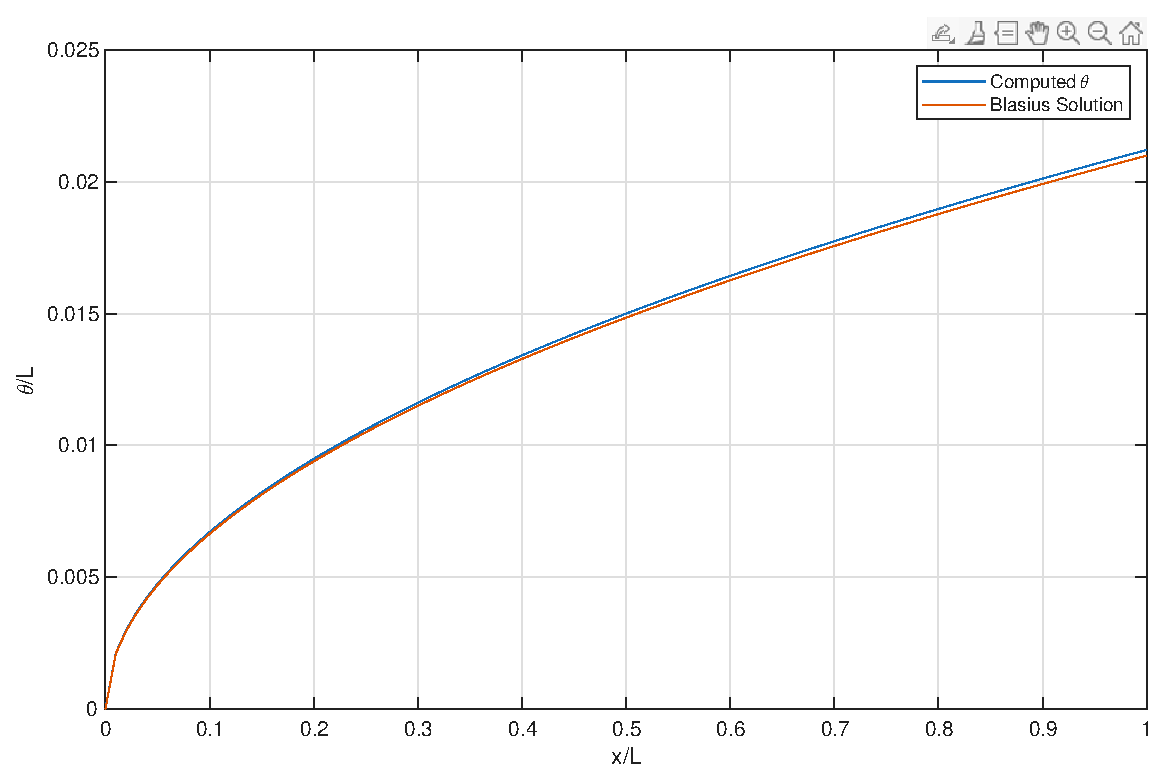
\includegraphics[width=0.75\linewidth]{Week_2/Exercise1.eps}
    \caption{Stream function plot for a point vortex. (Exercise 1)}
    \label{fig:placeholder}
\end{figure}
\begin{lstlisting}[language=Matlab, caption=The function to evaluate the contribution to the boundary layer integral. (Exercise 1)]
function f = ueintbit(xa, ua, xb, ub)
    ubar = (ua+ub)/2;
    du = ub-ua;
    dx = xb-xa;
    f = (ubar^5 + (5/6)*ubar^3 * du^2 + (1/16) * ubar * du^4)*dx;
end
\end{lstlisting}
\begin{lstlisting}[language=Matlab, caption={The script for plotting the boundary layer thickness of a flat plate with zero pressure gradient. (Exercise 1)}]
np = 101;
x = linspace(0,1,np);
u_ = 1*ones(1,np); %dimensionless velocity 

int = 0; % value of the integral 
theta_2 = zeros(1,np);  %theta squared at each position 
re_l = 1000;
for i=2:np
    int = int + ueintbit(x(i-1), u_(i-1), x(i), u_(i));
    theta_2(i) = (0.45/re_l) * u_(i)^(-6) * int;
end
analy = 0.664/re_l^(0.5) * x.^0.5;
theta = sqrt(theta_2);


figure;
plot(x, theta);
hold on;
plot(x, analy);
hold off;
xlabel('x/L');
ylabel('\theta/L');
legend('Computed \theta', 'Blausius Solution');
title('Comparison of Computed and Analytical Theta');
grid on;
print -deps2c Week_2/Exercise1.eps;


\end{lstlisting}

\end{document}